\section{Introduction}

So far we have mainly focused on models that handle \textbf{input and output of fixed size}. For example, in a convolutional neural network (CNN), we transform an input in the form of a matrix (image) into an output in the form of a vector (labels). However, the community has developed models that can handle variable-length structures, more specifically sequences, such as text, which is a sequence of strings.

Recurrent Neural Networks (RNNs) are flexible tools that can perform many different tasks, which can be classified as follows:

\begin{figure}[!htbp]
    \centering
    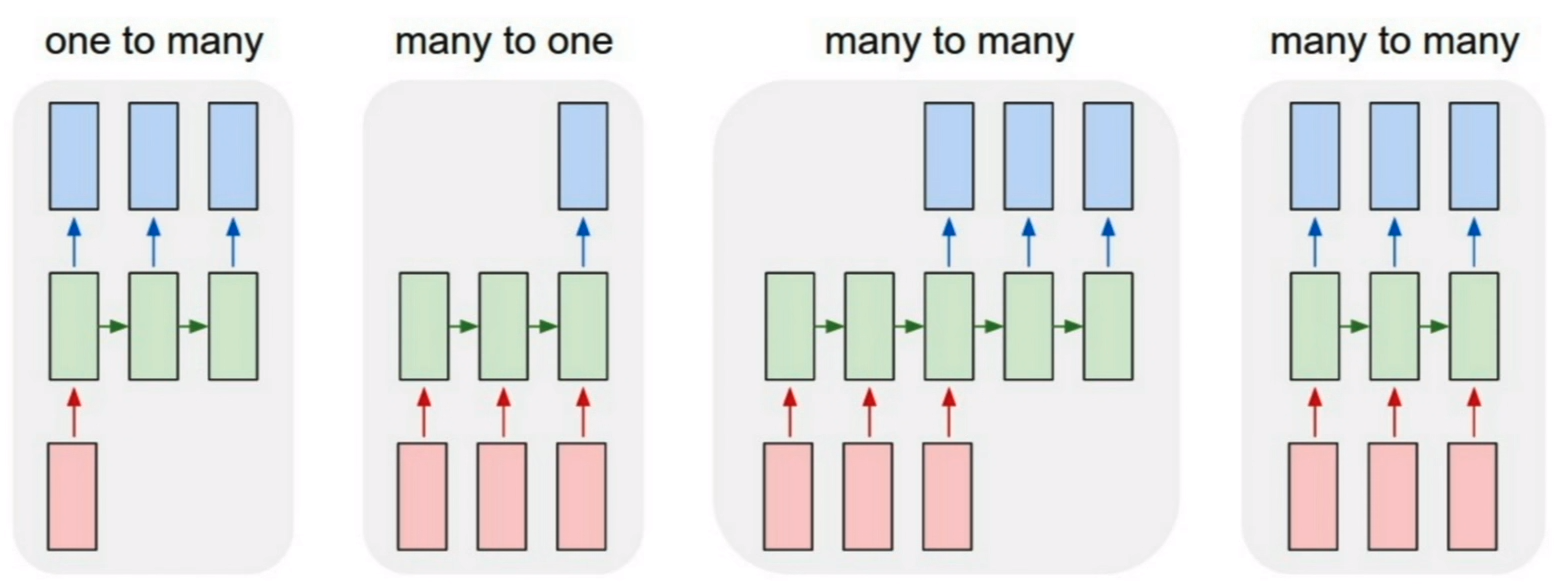
\includegraphics[width=\textwidth]{tikz/chapter6 - Types of RNN Models.png}
    \caption{{\color{red}\colorbox{pink}{Tikz TO-DO}} Diagrams of RNN Models}
\end{figure}

\subsection{Multiple2Single: Sentiment Analysis}

In the sentiment analysis, the model must classify a product, restaurant, or any other item as positive, neutral, or negative based on the reviews received. In this scenario, we provide the neural network with inputs of varying sizes. Each word is transformed into a \textbf{hidden representation that reflects the context and propagates through subsequent words}, as these words are not independent of each other. This propagation occurs unidirectionally, similar to a feedforward neural network. However, the main difference is that instead of mapping a single input to an output of fixed size, the model takes multiple inputs and produces a single label. Predictions are typically made about the last hidden state, which should include the context of previous words.

\subsection{Single2Multiple: Image Captioning}

In image captioning, the network is fed a fixed input (an image), but the output will have a variable length, since we want to produce a sentence describing the content of the image. In this case, the latent representation of the image obtained from a CNN is \textbf{combined with the latent representations of the words to model the dependencies between them}. This approach allows a single input to be mapped to multiple outputs, generating several words that describe the image.

\subsection{Multiple2Multiple: Machine Translation}

In machine translation, the task is to translate a sentence from one language to another. This problem involves both multiple inputs and multiple outputs. Each word in the input sentence is mapped to a hidden representation that takes into account the context of the preceding words. The neural network uses these representations to generate the translated sentence, word by word, \textbf{maintaining sequential dependencies between words}. This allows the model to produce an accurate translation that reflects the meaning of the original sentence.

\section{Vanilla RNN}

Recurrent neural networks are, in essence, \textbf{neural networks with cycles}.\\
Paper: \href{https://www.sciencedirect.com/science/article/pii/036402139090002E}{"Finding structure in time" (Jeffrey L. Elman)}


The RNN has a \textbf{recurrent design} in that it performs the same parametric function for each input ($x_t$, each marked with a timestep), while the output ($h_t$, the hidden representation marked with the corresponding timestep) depends on the previous computation ($h_{t-1}$). After producing the output, this is used to generate the hidden representation of the next RNN cell ($h_{t+1}$). To make a decision ($y_t$), a linear layer can be applied to the end of a cell, considering both the current input and the output learned from the previous input.

There are two types of representations for an RNN: the \textbf{Folded} representation, which is synthetic, and the \textbf{Unfolded} representation, which provides a more explicit description of the computations. Below is the architecture of the network in both representations:

\begin{figure}[!htbp]
    \centering
    \includegraphics[width = 0.9\linewidth]{tikz/chapter6 - RNN Architecture.pdf}
    \caption{{\color{red}\colorbox{pink}{Tikz To Refine}} RNN Architecture}
\end{figure}

The structure of an RNN cell, as shown in the figure above, has two inputs ($x_t$ and $h_{t-1}$) and can be represented mathematically as follows:

$$
h_t = f_w(x_t,h_{t-1}) = \text{tanh} \ W \begin{pmatrix}
x_t \\
h_{t-1}
\end{pmatrix} = \text{tanh}(W_xx_t + W_hh_{t-1})
$$

In this equation, $h_t$ represents the hidden state at time $t$, $x_t$ is the input at time $t$, $h_{t-1}$ is the previous hidden state, $W_x$ and $W_h$ are the weights associated with the current input and previous hidden state respectively. The function $\text{tanh}$ provides nonlinearity to the network. During training, $W$ weights are learned through the optimization process. For the prediction:
$$
y_t = \text{softmax}(W_y h_t + b_y)
$$
A peculiar aspect of RNNs is the \textbf{sharing of weights among different timesteps}. In these neural networks, the weights $W_x$, $W_h$ and $W_y$ are shared between different timestep iterations, allowing the model to capture \textbf{sequential dependencies within the data}.

So, the main differences between an RNN and an FNN include the sharing of weights between timesteps, the use of backpropagation variation for training and the presence of three different sets of weights: $W_x$, $W_h$ and $W_y$. In addition, \textbf{the problem of gradient vanishing is more severe} in RNNs than in feedforward networks, mainly because of the hyperbolic tangent function used as the activation function.


\subsection{Truncated BPTT (Backpropagation Through Time)}

To solve the problems described above, we use the Truncated BPTT algorithm, which is a more efficient technique when dealing with long sequences.

Imagine we need to train an RNN on a very long sequence, such as a sentence or a piece of music. The problem is that classical backpropagation through time can become very computationally expensive. The idea of Truncated BPTT is to simplify this process.

Instead of running the entire sequence through the network, we divide it into \textbf{smaller blocks of fixed length}. Each block is treated as a separate training unit. In this way, the network does not have to work with the whole sequence at once, but only with small chunks at a time, making training more efficient.

After presenting a block to the network, \textbf{backpropagation is performed only for a limited number of backward time steps}, rather than traversing the entire length of the sequence. This means that the network does not have to keep track of information too far back in time, reducing the computational cost of training.

To control how far back in time to go during backpropagation, we use two parameters, $k_1$ and $k_2$. $k_1$ determines the \textbf{length of the blocks} into which we divide the sequence, while $k_2$ defines the \textbf{number of time steps} over which to perform backpropagation within each block. The Truncated BPTT algorithm can be schematized as follows:

\begin{algorithm}
\renewcommand\thealgorithm{}
\caption{}
\begin{algorithmic}[1]
\STATE Present a sequence of $k_1$ timesteps of input and output pairs to the network.
\STATE Unroll the network then calculate and accumulate errors across $k_2$ timesteps.
\STATE Roll-up the network and update weights.
\STATE Repeat the process.
\end{algorithmic}
\end{algorithm}
Adjusting $k_1$ and $k_2$ allows us to balance the training speed and the network's ability to capture long-range time dependencies.

\section{Long Short-Term Memory (LSTM)}

It has been recognized that the vanilla RNN suffers from poor design in its individual cell, as efforts to enhance learning have not yielded significant improvements in vanishing gradient due to inherent limitations in the cell's design. To solve this problem, LSTM came into the stage. \\
Paper: \href{https://deeplearning.cs.cmu.edu/F23/document/readings/LSTM.pdf}{"Long Short-term Memory" (Sepp Hochreiter)}


The primary issue concerning the vanishing gradient problem stemmed from the fact that all computations involving dependencies between $h_t$ and $h_{t−1}$ must pass through a nonlinear function. An LSTM cell changed this property.

Firstly, LSTM cell not only produces the hidden state $h_t$, but it added another component, called \textbf{memory cell} ($c_t$), which is responsible for remembering and forgetting. This is based on the context of the input. This means that some of the previous information should be remembered while some of them should be forgotten and some of the new information should be added to the memory. Thus, it is not subject to matrix multiplication or squishing (non-linearity).

Furthermore, Inside a LSTM cell, three differents parametric components, called \textbf{gates}, were added. We have listed them following the cell's structure order:

\begin{remark}{myred}{myred!20}
Magari qui da rifare con tre "remark" con vari colori e nel disegno farli uguali per far capire meglio.
+ mettere a posto parentesi nelle formule
\end{remark}

\textbf{Forget gate}: can modulate the memory cell's self-recurrent
connection, allowing the cell to remember or forget its previous state, as needed.  

Its ouptut $f_t$ is computed by the sigmoid, applied to the input $x_t$ and the previous dependency $h_{t-1}$, and it is associated to its own parameters $W_f$. $$ f_t = \sigma(W_f
\begin{pmatrix}
x_t \\
h_{t-1}
\end{pmatrix} + b_f)
$$

    
\textbf{Input gate}: can allow incoming signal ($x_t$ and $h_{t-1}$) to alter the state of the memory cell or block it.

Its output $i_t$ is computed by the sigmoid, applied to the input $x_t$ and the previous dependency $h_{t-1}$, and it is associated to its own parameters $W_i$. $$ i_t = \sigma(W_i
\begin{pmatrix}
x_t \\
h_{t-1}
\end{pmatrix} + b_i)
$$

$i_t$ is used as a trade-off between the information passing through the current input ($x_t$ and $h_{t-1}$) and the information encoded by the previous cell ($c_{t-1}$). The model also determines what should not be forgotten in the previous cell state by employing $f_t$ and adding the output:

$$c_t = f_t \circ c_{t-1} + i_t \circ g_t $$


-----
Possiamo interpretare l'equazione nel seguente modo:
\begin{itemize}
    \item \( f_t \circ c_{t-1}: \) 
    \begin{itemize}
        \item Questo termine rappresenta il "forget gate" \( f_t \) moltiplicato per lo stato precedente della cella \( c_{t-1} \).
        \item Il forget gate decide quanto dello stato precedente della cella \( c_{t-1} \) deve essere dimenticato o mantenuto per il prossimo stato \( c_t \).
    \end{itemize}
    \item \( i_t \circ g_t: \)
    \begin{itemize}
        \item Questo termine rappresenta l'"input gate" \( i_t \) moltiplicato per il valore dell'input modulation \( g_t \).
        \item Questo determina quanto della nuova informazione \( g_t \) deve essere aggiunta allo stato della cella \( c_t \).
    \end{itemize}
    \item \( c_t = \)
    \begin{itemize}
        \item Quindi, \( c_t \) è calcolato combinando una frazione dello stato precedente della cella, determinata dal forget gate \( f_t \),
        \item e una frazione della nuova informazione, determinata dall'input gate \( i_t \) e dall'input modulation \( g_t \).
    \end{itemize}
\end{itemize}

In breve, il forget gate modula quanto dello stato precedente conservare, mentre l'input gate modula quanto della nuova informazione deve essere aggiunta allo stato della cella.
-----

Notice that although we have a bounce of non linearity functions, the computations to update the value of the cell ($c_t$) is \textbf{linear}, thus Gradient flow from $c_t$ to $c_{t-1}$ only involves backpropagating through addition and element-wise multiplication, not matrix multiplication or non-linearity.


    
\textbf{Output gate}: can allow the state of the memory cell ($c_t$) to have an effect on other neurons, thus it affects the output of the LSTM uint ($h_t$)
    
First, a sigmoid layer decides what parts of the cell state ($c_t$) the model is going to output (associated its own parameters $W_o$).

$$ o_t = \sigma(W_o
\begin{pmatrix}
x_t \\
h_{t-1}
\end{pmatrix} + b_o)
$$

Then, a tanh layer is used on the cell state to squash the values between -1 and 1, which is finally multiplied by the sigmoid gate output.

$$h_t = o_t \circ \text{tahn } c_{t} $$


\begin{figure}[!htbp]
    \centering
    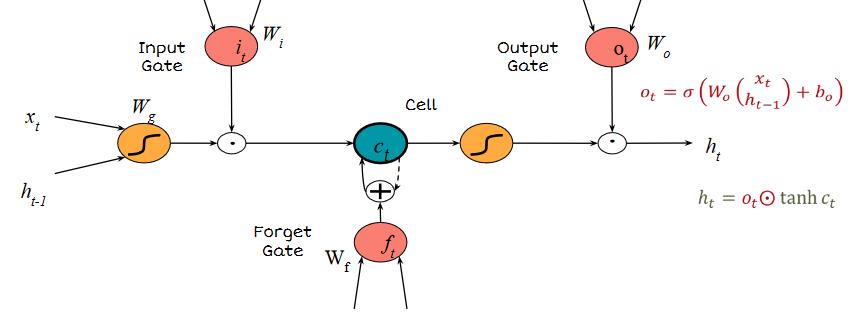
\includegraphics[width=\linewidth]{tikz/chapter6 - LSTM.png}
    \caption{{\color{red}\colorbox{pink}{Tikz TO-DO}} LSTM Cell Structure}
\end{figure}


\section{Gated Recurrent Unit (GRU)}

When the community began applying LSTM models to various tasks such as captioning, it became evident that the network was overly complex. GRU networks address this complexity by simplifying the LSTM cell, removing one of its gates, as each of which has its own set of parameters, and the usage of the cell state $c_t$. Despite having just two gates, the model is resilient enough to the vanishing gradient. Furthermore, information flow will be stored just in the hidden state $h_t$.\\
Paper: \href{https://arxiv.org/pdf/1406.1078}{"Learning Phrase Representations using RNN Encoder–Decoder
for Statistical Machine Translation" (Cho et al.)}


The gates used in the GRU model are:

\textbf{Reset gate}:  to decide how much of the past information to forget.

Its output $r_t$ is computed by the sigmoid, applied to the input $x_t$ and the previous hidden stae $h_{t-1}$, and it is associated to its own parameters $W_r$. $$ r_t = \sigma(W_r
\begin{pmatrix}
x_t \\
h_{t-1}
\end{pmatrix} + b_t)
$$

An important change in LSTM cell design occurs in the GRU cell, where the computation of the vanilla RNN output no longer relies solely on the full information from the previous hidden state $h_{t−1}$, but instead on a "restricted flow" determined by $r_t$:

$$ h^{'}_t = \text{tahn }W(
\begin{pmatrix}
x_t \\
r_t \cdot h_{t-1}
\end{pmatrix})
$$



\textbf{Update gate}: helps the model to determine how much of
the past information (from previous time steps) needs to be passed along to the future.

Its output $z_t$ is computed by the sigmoid, applied to the input $x_t$ and the previous hidden state $h_{t-1}$, and it is associated to its own parameters $W_z$. $$ z_t = \sigma(W_z
\begin{pmatrix}
x_t \\
h_{t-1}
\end{pmatrix} + b_z)
$$

The hidden representation is computed by an additional dot product: 

$$h_t = (1-z_t)\cdot h_{t-1}+z_t \cdot h^{'}_t$$

\begin{figure}[!htbp]
    \centering
    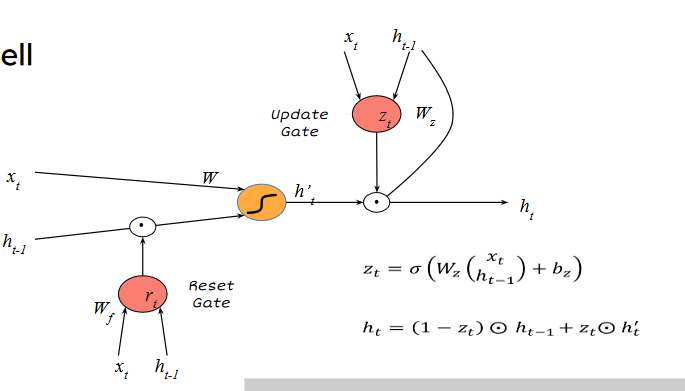
\includegraphics[width=\linewidth]{tikz/chapter6 - GRU.png}
    \caption{{\color{red}\colorbox{pink}{Tikz TO-DO}} GRU Cell Structure}
\end{figure}

In complex applications, single-layer architectures cannot be used. Therefore, more advanced structures such as \textbf{Bidirectional RNNs} are used. This type of model not only improves the modeling of temporal dependencies between words in a sentence, but also processes the input sequence both forward and backward. When applying the softmax function, it is necessary to concatenate the hidden states of both RNNs. This approach is widely used in speech recognition.